% Options for packages loaded elsewhere
\PassOptionsToPackage{unicode}{hyperref}
\PassOptionsToPackage{hyphens}{url}
%
\documentclass[
]{article}
\usepackage{lmodern}
\usepackage{amsmath}
\usepackage{ifxetex,ifluatex}
\ifnum 0\ifxetex 1\fi\ifluatex 1\fi=0 % if pdftex
  \usepackage[T1]{fontenc}
  \usepackage[utf8]{inputenc}
  \usepackage{textcomp} % provide euro and other symbols
  \usepackage{amssymb}
\else % if luatex or xetex
  \usepackage{unicode-math}
  \defaultfontfeatures{Scale=MatchLowercase}
  \defaultfontfeatures[\rmfamily]{Ligatures=TeX,Scale=1}
\fi
% Use upquote if available, for straight quotes in verbatim environments
\IfFileExists{upquote.sty}{\usepackage{upquote}}{}
\IfFileExists{microtype.sty}{% use microtype if available
  \usepackage[]{microtype}
  \UseMicrotypeSet[protrusion]{basicmath} % disable protrusion for tt fonts
}{}
\makeatletter
\@ifundefined{KOMAClassName}{% if non-KOMA class
  \IfFileExists{parskip.sty}{%
    \usepackage{parskip}
  }{% else
    \setlength{\parindent}{0pt}
    \setlength{\parskip}{6pt plus 2pt minus 1pt}}
}{% if KOMA class
  \KOMAoptions{parskip=half}}
\makeatother
\usepackage{xcolor}
\IfFileExists{xurl.sty}{\usepackage{xurl}}{} % add URL line breaks if available
\IfFileExists{bookmark.sty}{\usepackage{bookmark}}{\usepackage{hyperref}}
\hypersetup{
  pdftitle={VISTAS - Visualising Industry Skill TAlent Shifts - User Guide},
  pdfauthor={Amos Lau; Cheryl Pay; Louis Chong},
  hidelinks,
  pdfcreator={LaTeX via pandoc}}
\urlstyle{same} % disable monospaced font for URLs
\usepackage[margin=1in]{geometry}
\usepackage{graphicx}
\makeatletter
\def\maxwidth{\ifdim\Gin@nat@width>\linewidth\linewidth\else\Gin@nat@width\fi}
\def\maxheight{\ifdim\Gin@nat@height>\textheight\textheight\else\Gin@nat@height\fi}
\makeatother
% Scale images if necessary, so that they will not overflow the page
% margins by default, and it is still possible to overwrite the defaults
% using explicit options in \includegraphics[width, height, ...]{}
\setkeys{Gin}{width=\maxwidth,height=\maxheight,keepaspectratio}
% Set default figure placement to htbp
\makeatletter
\def\fps@figure{htbp}
\makeatother
\setlength{\emergencystretch}{3em} % prevent overfull lines
\providecommand{\tightlist}{%
  \setlength{\itemsep}{0pt}\setlength{\parskip}{0pt}}
\setcounter{secnumdepth}{-\maxdimen} % remove section numbering
\ifluatex
  \usepackage{selnolig}  % disable illegal ligatures
\fi

\title{VISTAS - Visualising Industry Skill TAlent Shifts - User Guide}
\author{Amos Lau \and Cheryl Pay \and Louis Chong}
\date{4/12/2021}

\begin{document}
\maketitle

\hypertarget{user-guide-for-vistas-visualising-industry-skill-talent-shifts}{%
\subsection{User Guide for VISTAS (Visualising Industry Skill TAlent
Shifts)}\label{user-guide-for-vistas-visualising-industry-skill-talent-shifts}}

\hypertarget{introduction-page}{%
\subsubsection{1. Introduction Page}\label{introduction-page}}

On this page, there is a description of the application and cards that
link to the various visualisation tabs.

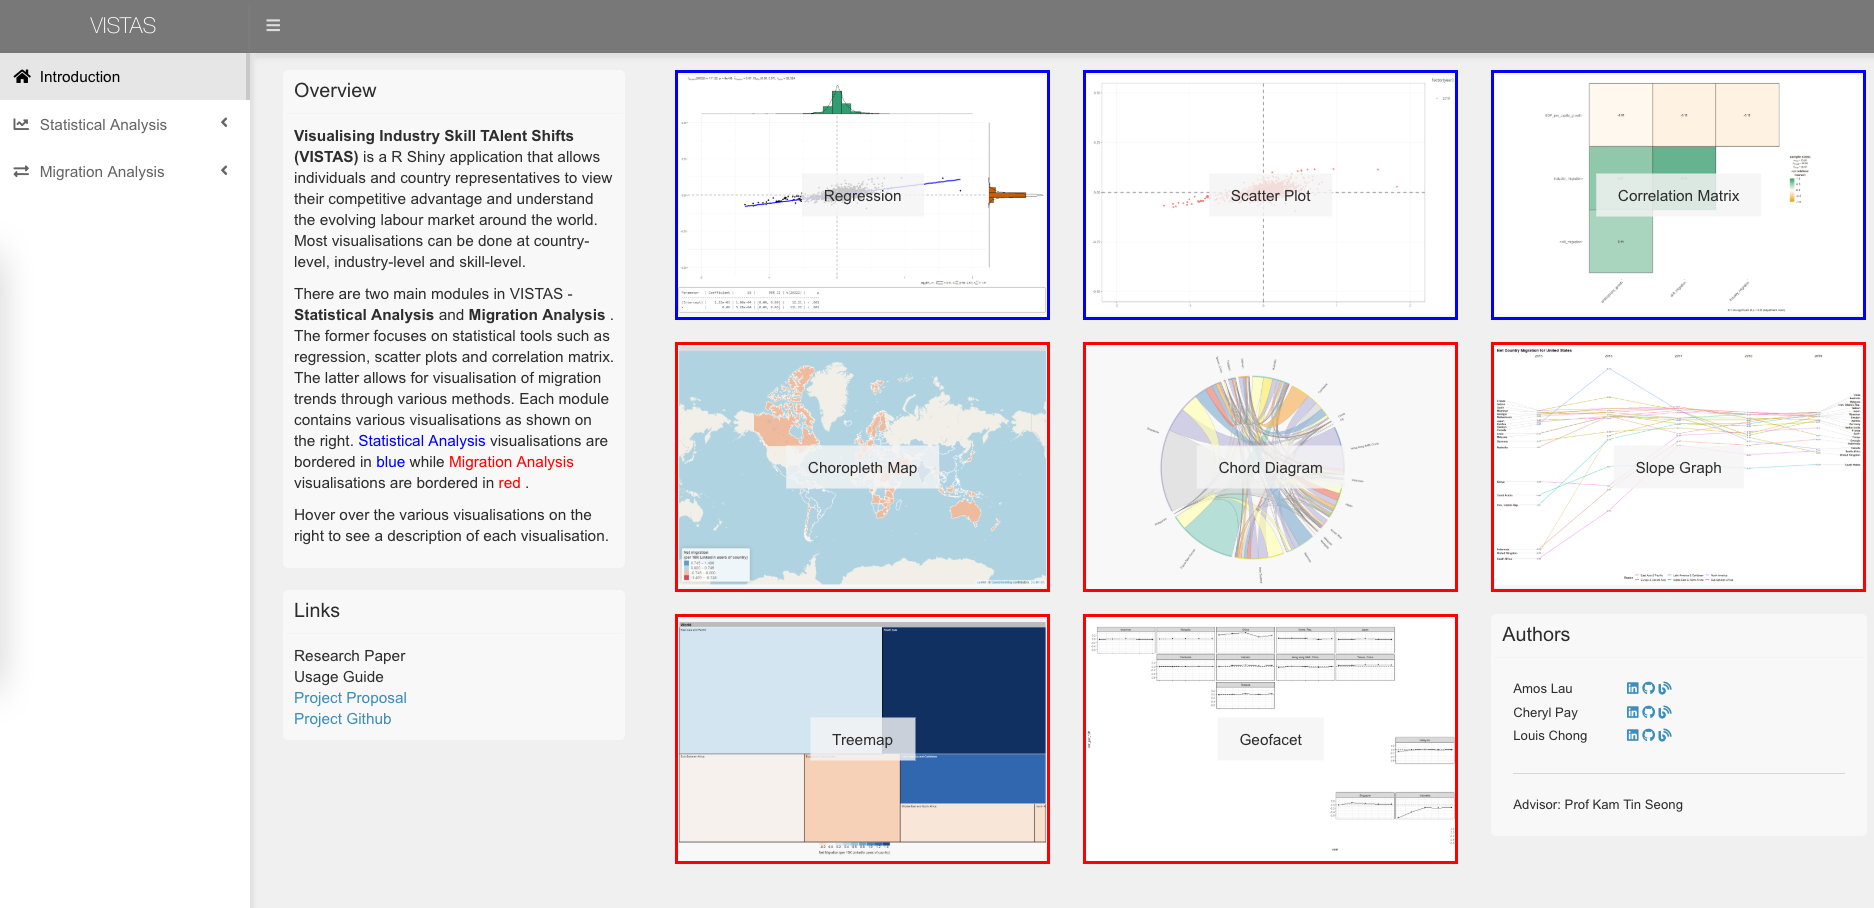
\includegraphics[width=1\textwidth,height=\textheight]{images/01_introduction.png}

When you hover over a card, the card flips to show a description and
link to the visualisation. Below, the card for the choropleth map is
flipped.

\includegraphics{images/02_hover-01.png}

On the side panel, a tooltip also appears when you hover over each
sub-tabs. Below, the tooltip for scatter plot is shown when you move
your cursor to Scatter Plot.

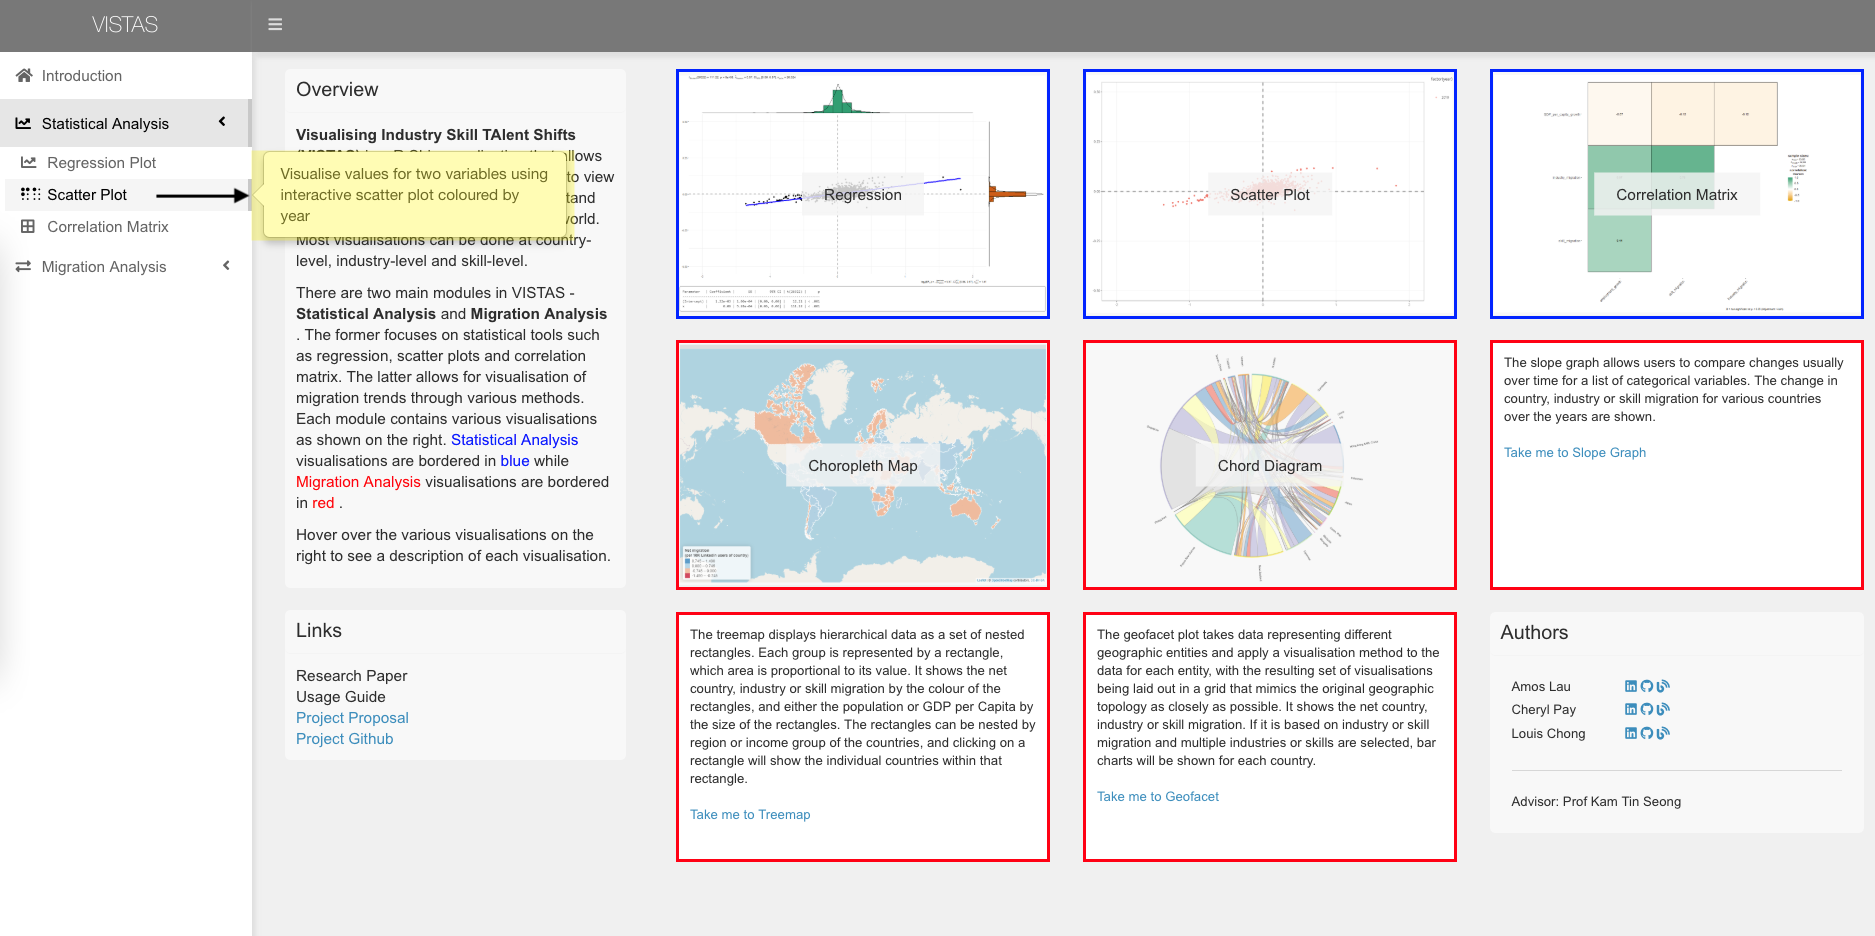
\includegraphics{images/03-tooltip.png}

Across each tab, there are two help buttons and many tooltips.

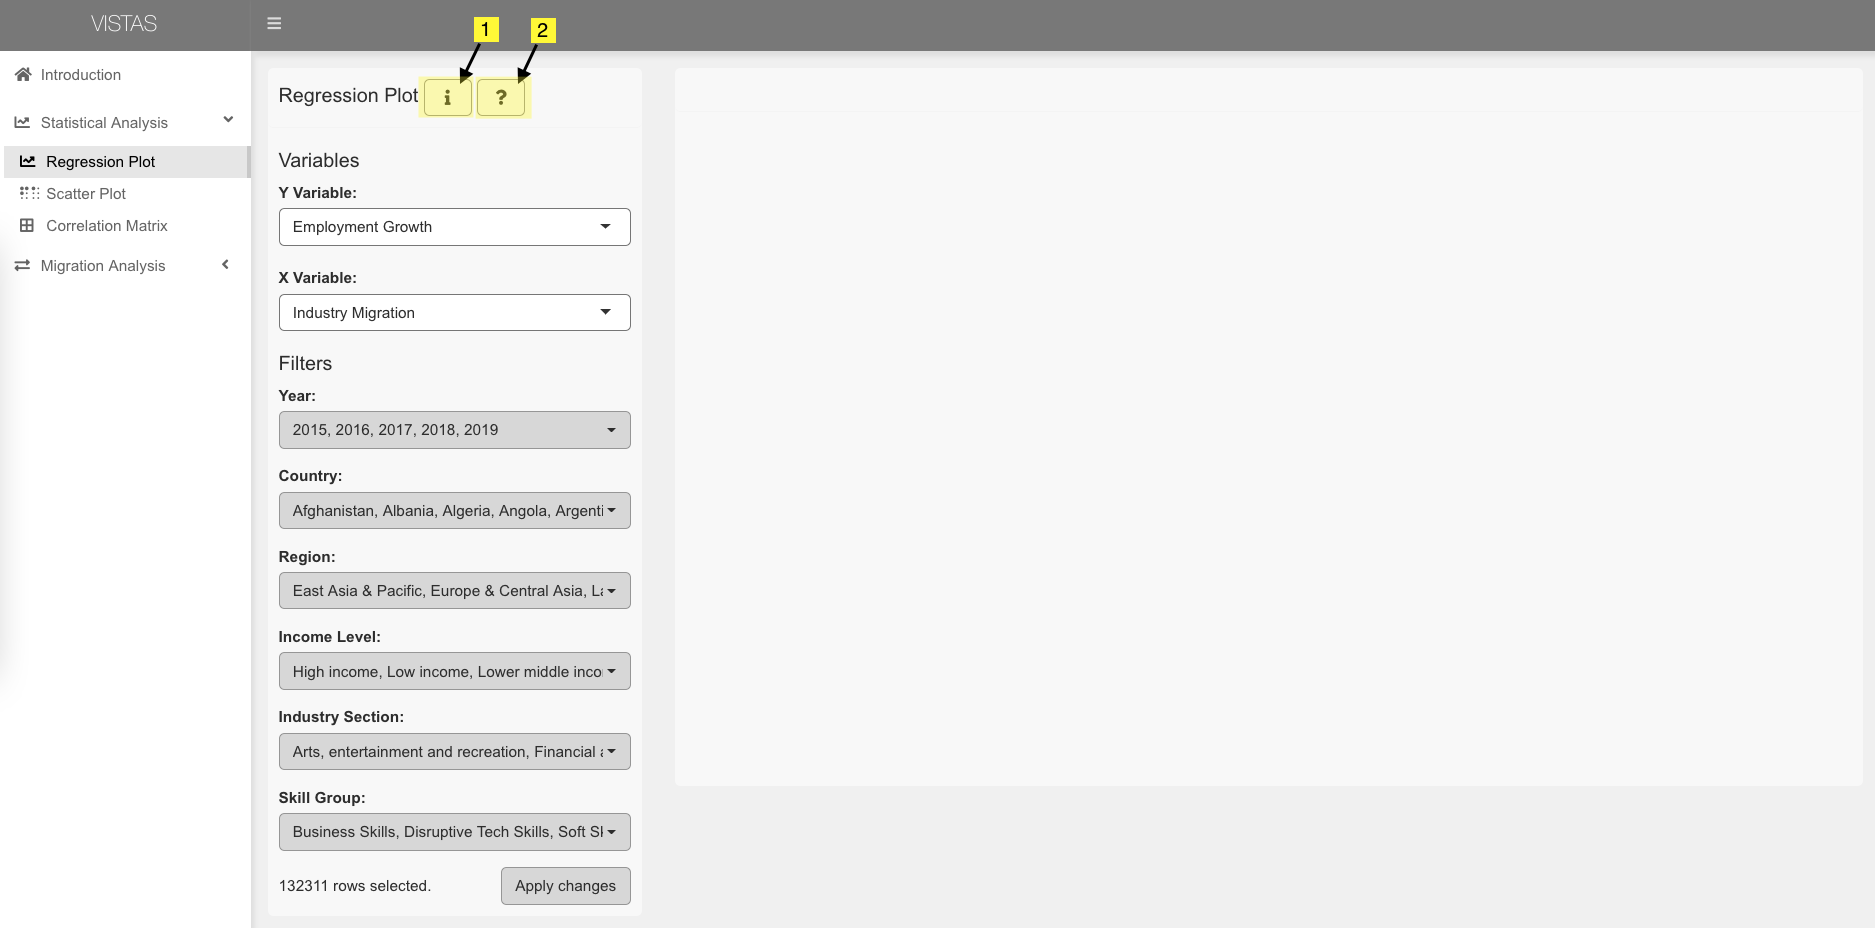
\includegraphics{images/04-info-user-guide.png}

\begin{enumerate}
\def\labelenumi{\arabic{enumi}.}
\item
  When the \textbf{i} button is clicked, a description of the
  visualisation will pop up.

  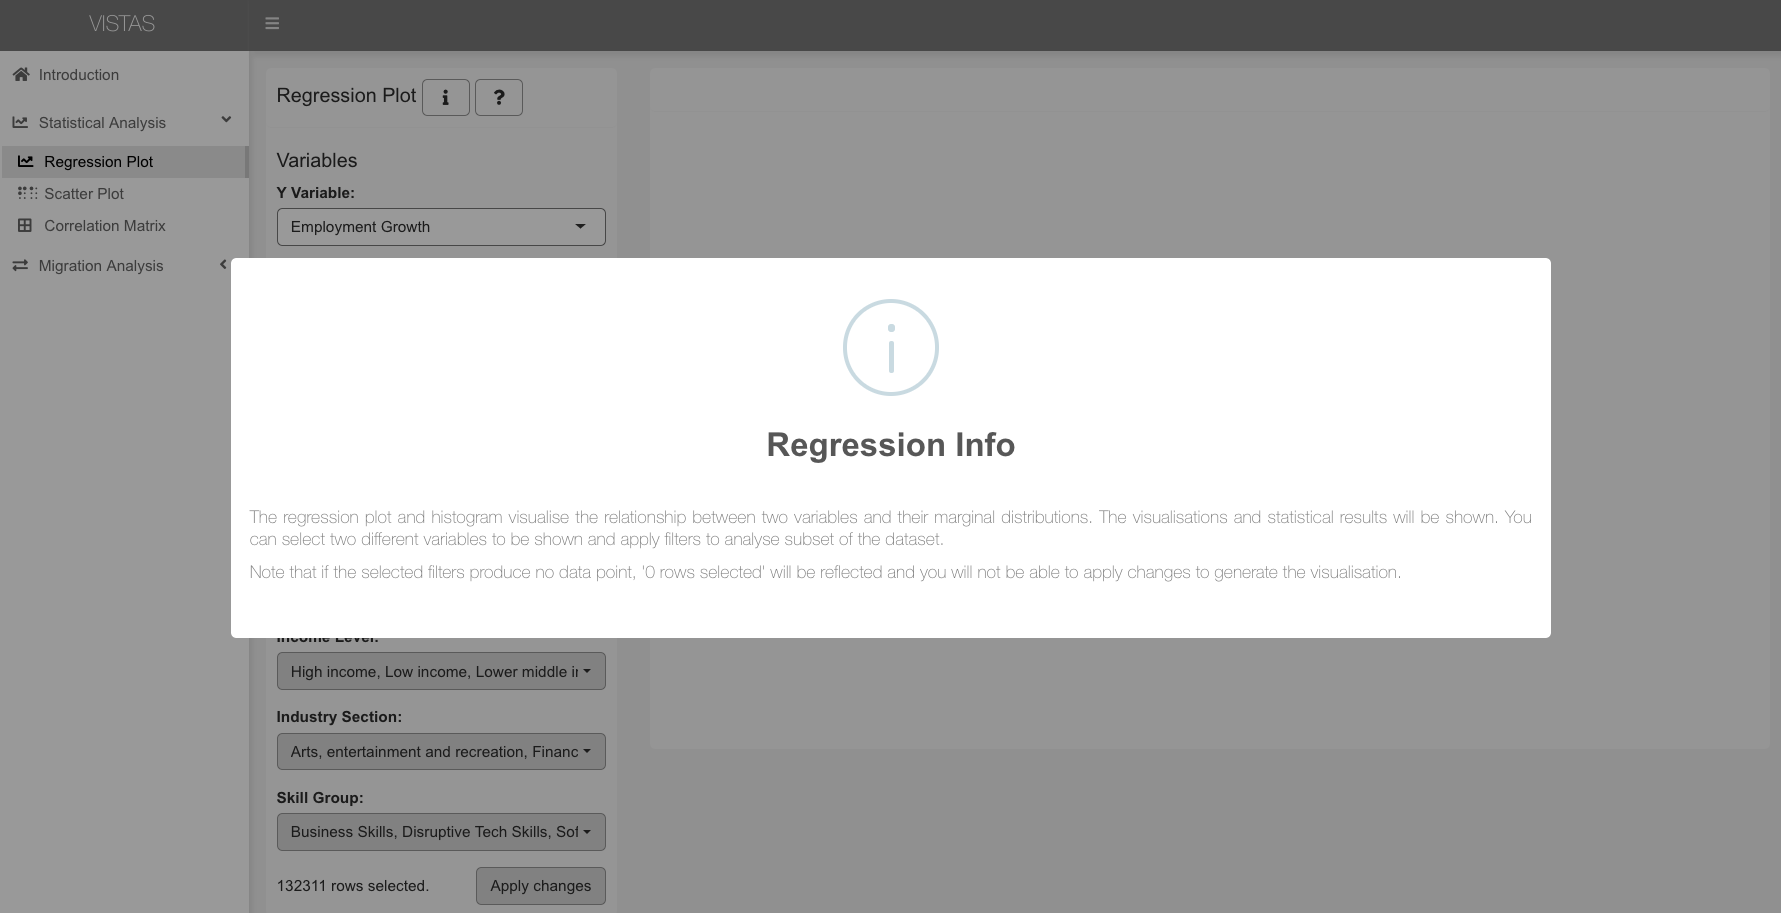
\includegraphics[width=0.8\textwidth,height=\textheight]{images/04-regression-info.png}
\item
  When the \textbf{?} button is clicked, a guide on selecting the inputs
  for the visualisation will pop up.

  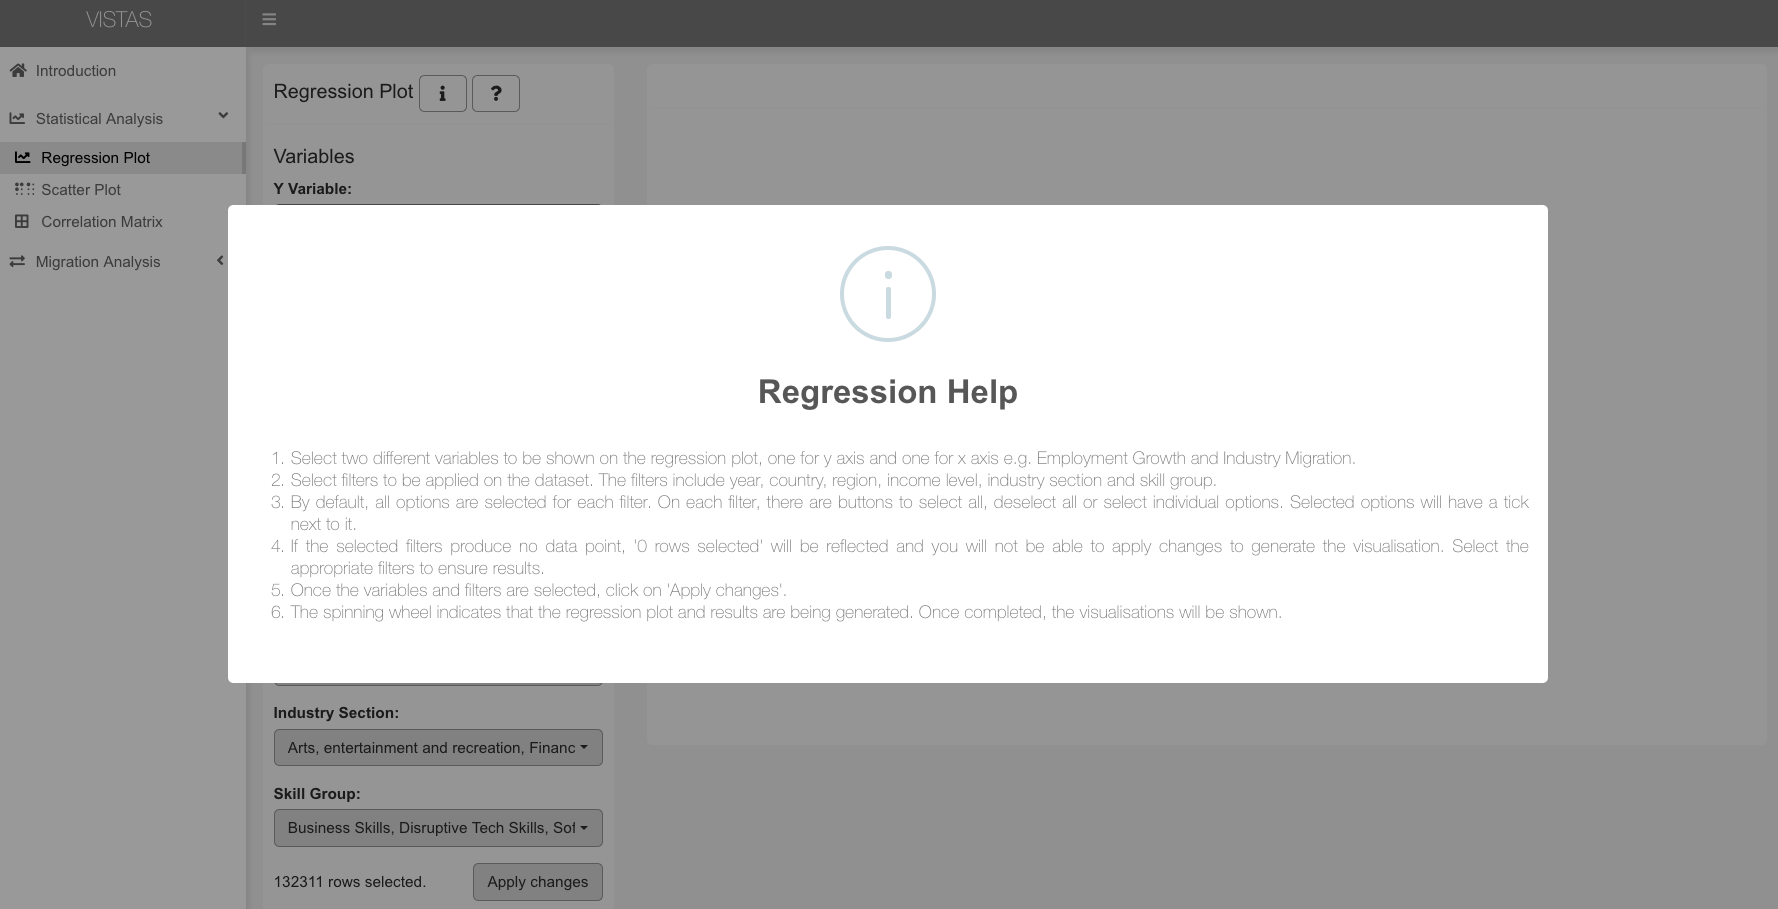
\includegraphics[width=0.8\textwidth,height=\textheight]{images/05-regression-help.png}
\item
  Spinning wheels are added to signify that the visualisations are being
  generated.

  \includegraphics[width=0.8\textwidth,height=\textheight]{images/07-spinning wheel-01.png}\includegraphics{}
\item
  When you hover over the input labels, a tooltip will appear to
  describe its significance.

  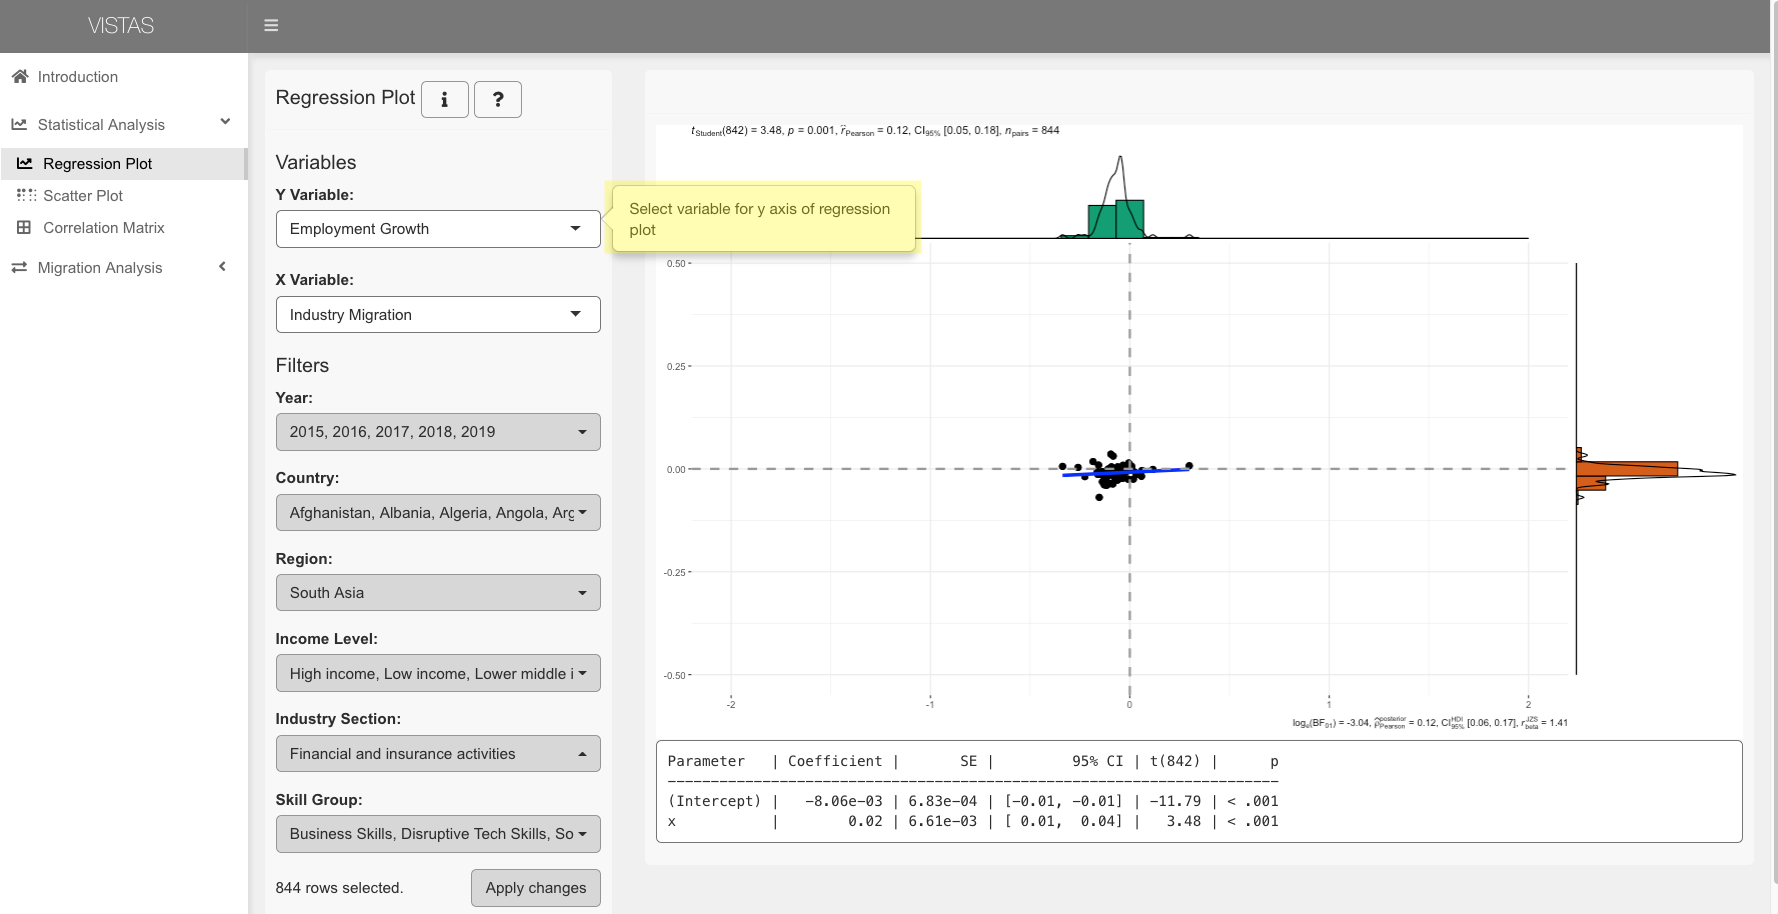
\includegraphics[width=0.8\textwidth,height=\textheight]{images/06-regression-input-tooltip.png}
\end{enumerate}

\hypertarget{statistical-analysis}{%
\subsubsection{2. Statistical Analysis}\label{statistical-analysis}}

This tab has three sub-tabs for regression, scatter plot and correlation
matrix. Each sub-tab has their own set of user inputs available.

\hypertarget{regression}{%
\paragraph{2.1 Regression}\label{regression}}

\includegraphics[width=1\textwidth,height=\textheight]{images/06-reg-01.png}

\begin{enumerate}
\def\labelenumi{\arabic{enumi}.}
\item
  Click on Regression in the navigation bar.
\item
  Select the variable to plot on the y axis e.g.~Employment Growth.
\item
  Select the variable to plot on the x axis e.g.~Industry Migration.
\item
  Select filters to be applied on the dataset. The filters include year,
  country, region, income level, industry section and skill group.

  By default, all options are selected for each filter. On each filter,
  there are buttons to select all, deselect all or select individual
  options. Selected options will have a tick next to it.
\item
  If the selected filters produce no data point, `0 rows selected' will
  be reflected and you will not be able to apply changes to generate the
  visualisation. Amend your filters to ensure results.
\item
  Click on `Apply changes' to generate the Regression Plot.

  \emph{The spinning wheel indicates that the correlation matrix is
  being generated.} Once completed, the visualisation will be shown.
\end{enumerate}

\hypertarget{scatterplot}{%
\paragraph{2.2 Scatterplot}\label{scatterplot}}

\includegraphics{images/08-scatter-01.png}

\begin{enumerate}
\def\labelenumi{\arabic{enumi}.}
\item
  Click on Scatter Plot in the navigation bar.
\item
  Select the variable to plot on the y axis e.g.~Employment Growth.
\item
  Select the variable to plot on the x axis e.g.~Industry Migration.
\item
  Select filters to be applied on the dataset. The filters include year,
  country, region, income level, industry section and skill group.

  By default, all options are selected for each filter. On each filter,
  there are buttons to select all, deselect all or select individual
  options. Selected options will have a tick next to it.
\item
  If the selected filters produce no data point, `0 rows selected' will
  be reflected and you will not be able to apply changes to generate the
  visualisation. Select the appropriate filters to ensure results.
\item
  Once the variables and filters are selected, click on `Apply changes'.
\item
  Hover over each point on the interactive scatter plot to find out its
  values i.e.~x variable, y variable, year, country, industry and skill.
\item
  There are buttons on the interactive scatter plot to carry out actions
  e.g.~download plot as png, zoom, select.

  \emph{The spinning wheel indicates that the correlation matrix is
  being generated.} Once completed, the visualisation will be shown.
\end{enumerate}

\hypertarget{correlation-matrix}{%
\paragraph{2.3 Correlation Matrix}\label{correlation-matrix}}

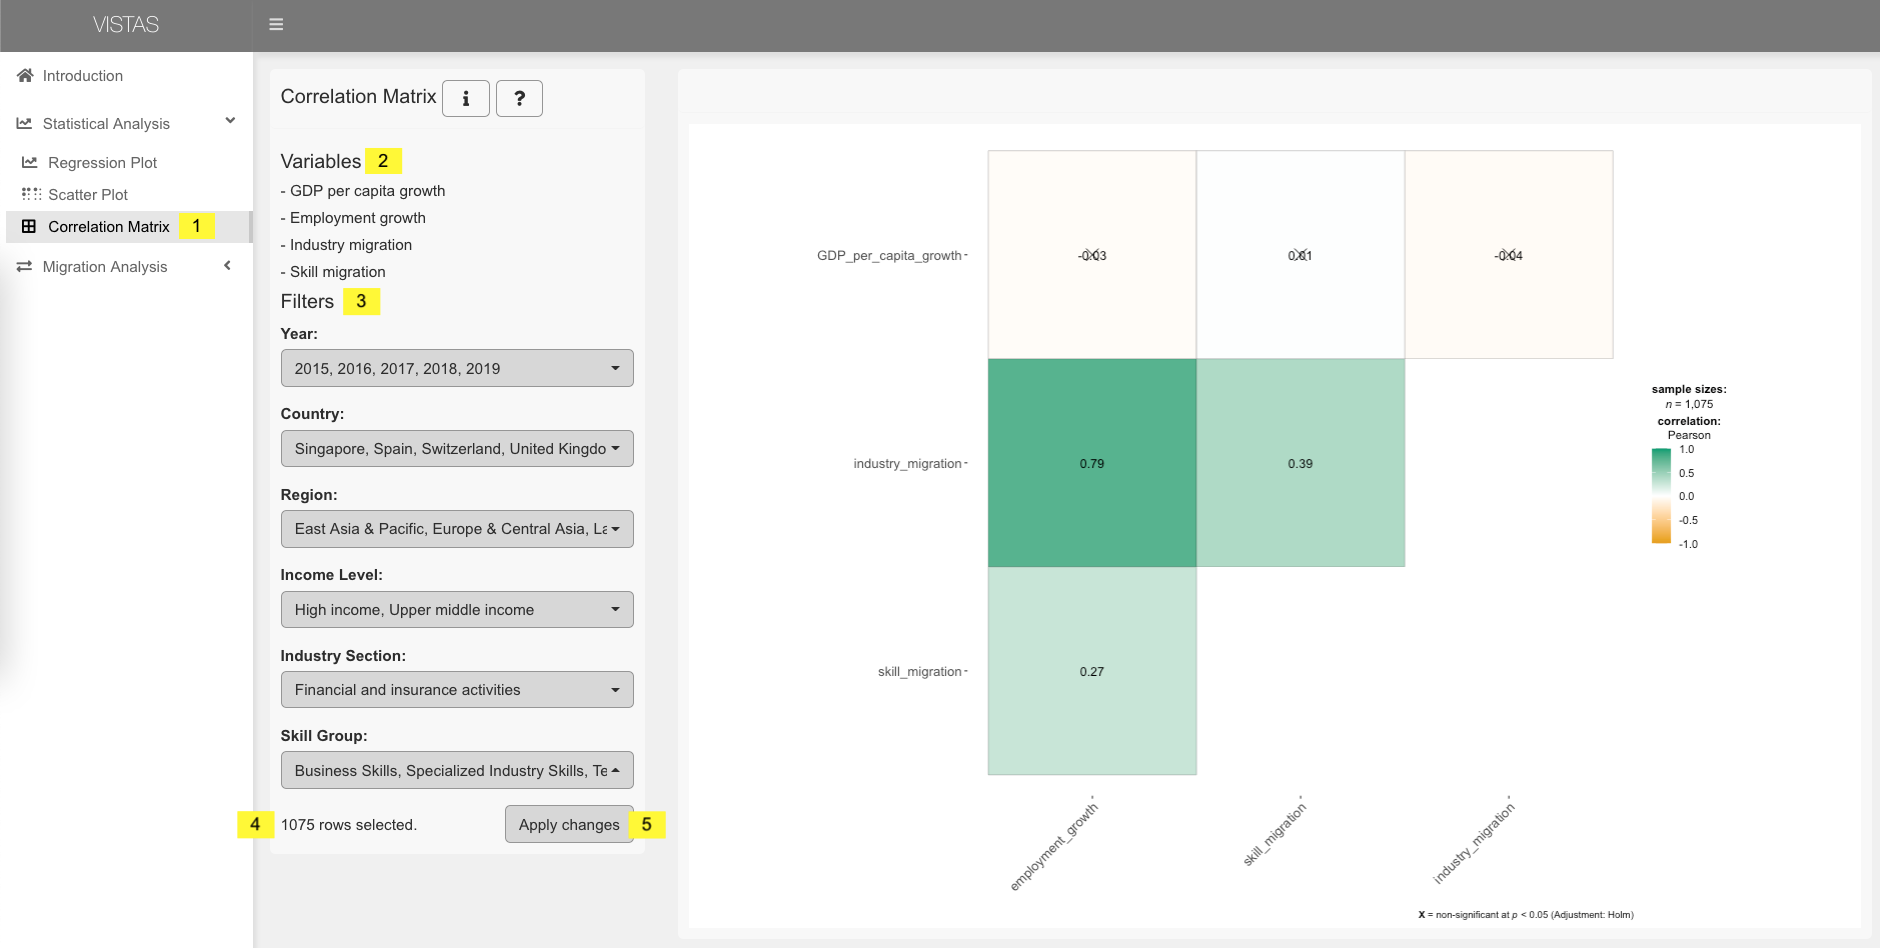
\includegraphics{images/09-correlation.png}

\begin{enumerate}
\def\labelenumi{\arabic{enumi}.}
\item
  Click on Correlation Matrix in the navigation bar.
\item
  Four variables are used for the correlation matrix i.e.~GDP per capita
  growth, Employment growth, Industry migration and Skill migration.
\item
  Select filters to be applied on the dataset. The filters include year,
  country, region, income level, industry section and skill group.

  By default, all options are selected for each filter. On each filter,
  there are buttons to select all, deselect all or select individual
  options. Selected options will have a tick next to it.
\item
  If the selected filters produce no data point, `0 rows selected' will
  be reflected and you will not be able to apply changes to generate the
  visualisation. Select the appropriate filters to ensure results.
\item
  Once the variables and filters are selected, click on `Apply changes'.

  \emph{The spinning wheel indicates that the correlation matrix is
  being generated.} Once completed, the visualisation will be shown.
\end{enumerate}

\hypertarget{migration-analysis}{%
\subsubsection{3. Migration Analysis}\label{migration-analysis}}

\hypertarget{choropleth-map}{%
\paragraph{3.1 Choropleth Map}\label{choropleth-map}}

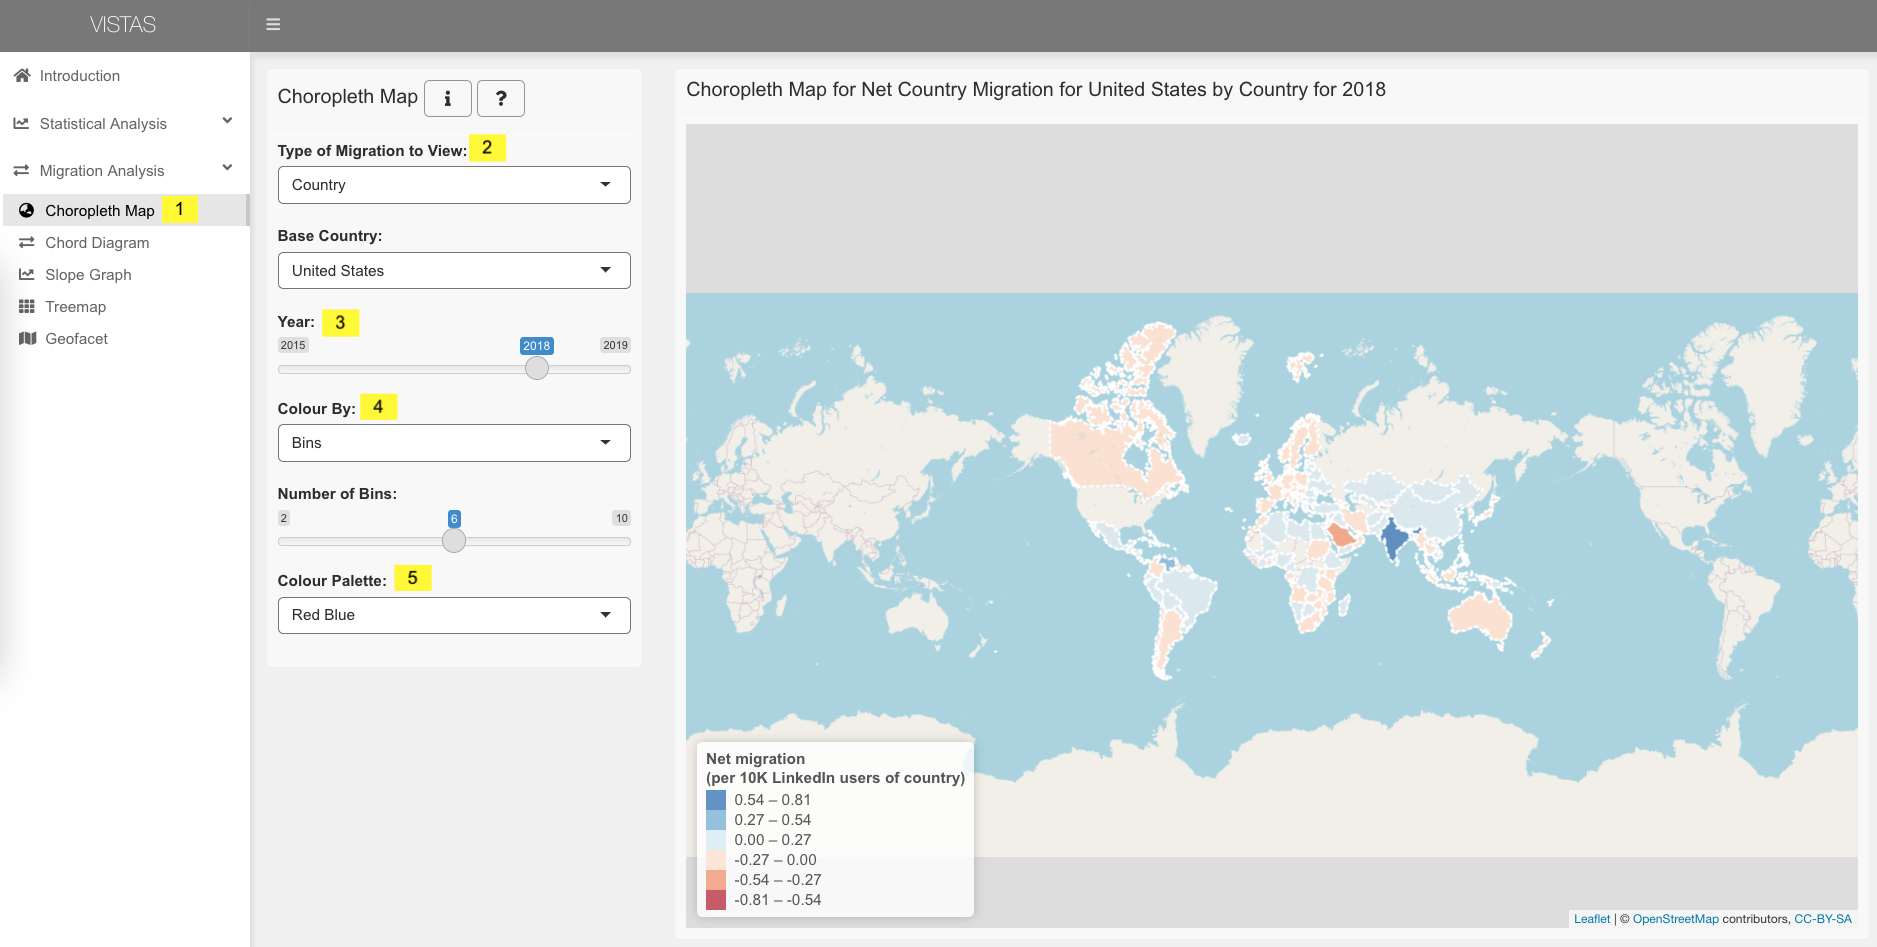
\includegraphics{images/10-choropleth.png}

\begin{enumerate}
\def\labelenumi{\arabic{enumi}.}
\item
  Click on Choropleth Map in the navigation bar.
\item
  Select Type of Migration to View from the dropdown -- Country,
  Industry or Skill.

  \begin{itemize}
  \item
    When Country is selected, you must further select Base Country
    i.e.~the country you want to see the net migration for. The dropdown
    list is sorted by Region then alphabetical order.
  \item
    When Industry is selected, you must further select the Industries
    you want to see the net migration for.
  \item
    When Skills is selected, you must further select the Skills you want
    to see the net migration for.
  \end{itemize}
\item
  Select Year on the slider as the data covers years 2015 -- 2019 (both
  years included).
\item
  Select Colour by from the dropdown. This variable determines the
  shades you see on the map.

  \begin{itemize}
  \item
    When Bins is selected, you can further indicate the number of bins.
  \item
    When Quantile is selected, you can further indicate the number of
    quantiles.
  \item
    When Numeric is selected, no further options are available.
  \end{itemize}
\item
  Select Colour Palette to watch the colours of the choropleth map
  change.
\end{enumerate}

\hypertarget{chord-diagram}{%
\paragraph{3.2 Chord Diagram}\label{chord-diagram}}

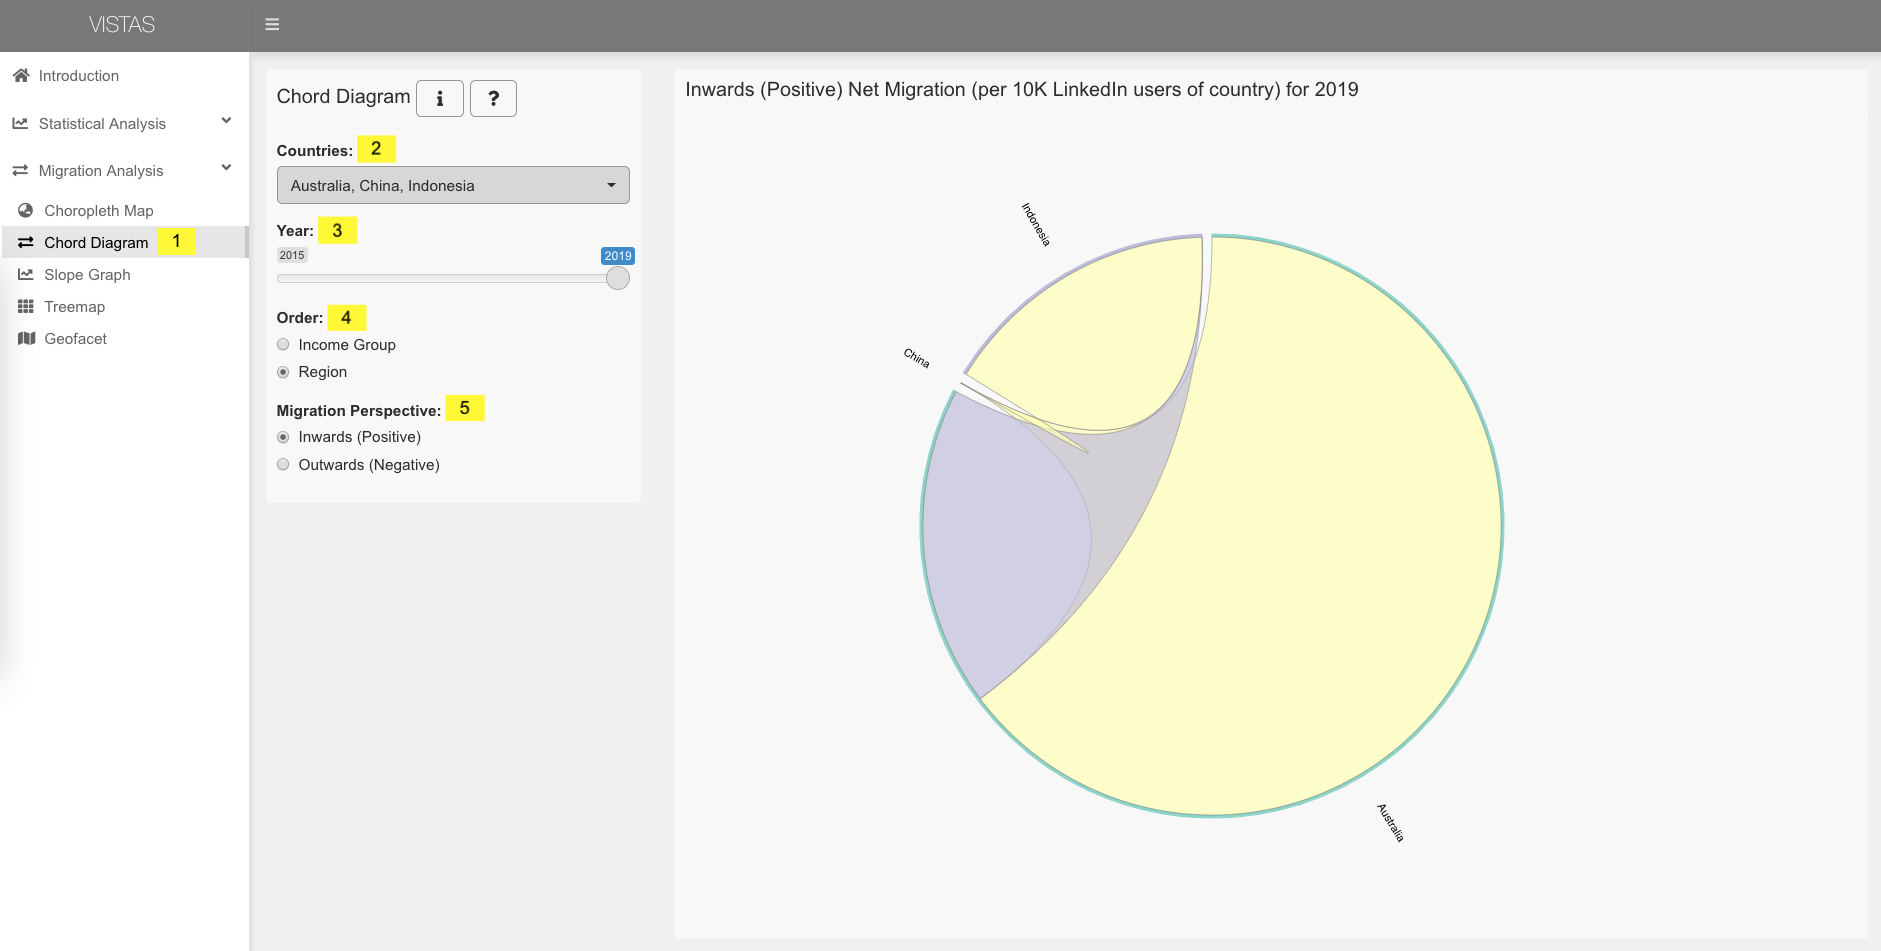
\includegraphics{images/11-chord.png}

\begin{enumerate}
\def\labelenumi{\arabic{enumi}.}
\tightlist
\item
  Click on the Chord Diagram in the navigation bar.
\item
  Select at least three countries from the dropdown list for Countries.
\item
  Select Year on the slider as the data covers years 2015 -- 2019 (both
  years included).
\item
  Select Order by Income Group or Region.
\item
  Select Migration Perspective inwards or outwards.
\end{enumerate}

\hypertarget{slope-graph}{%
\paragraph{3.3 Slope Graph}\label{slope-graph}}

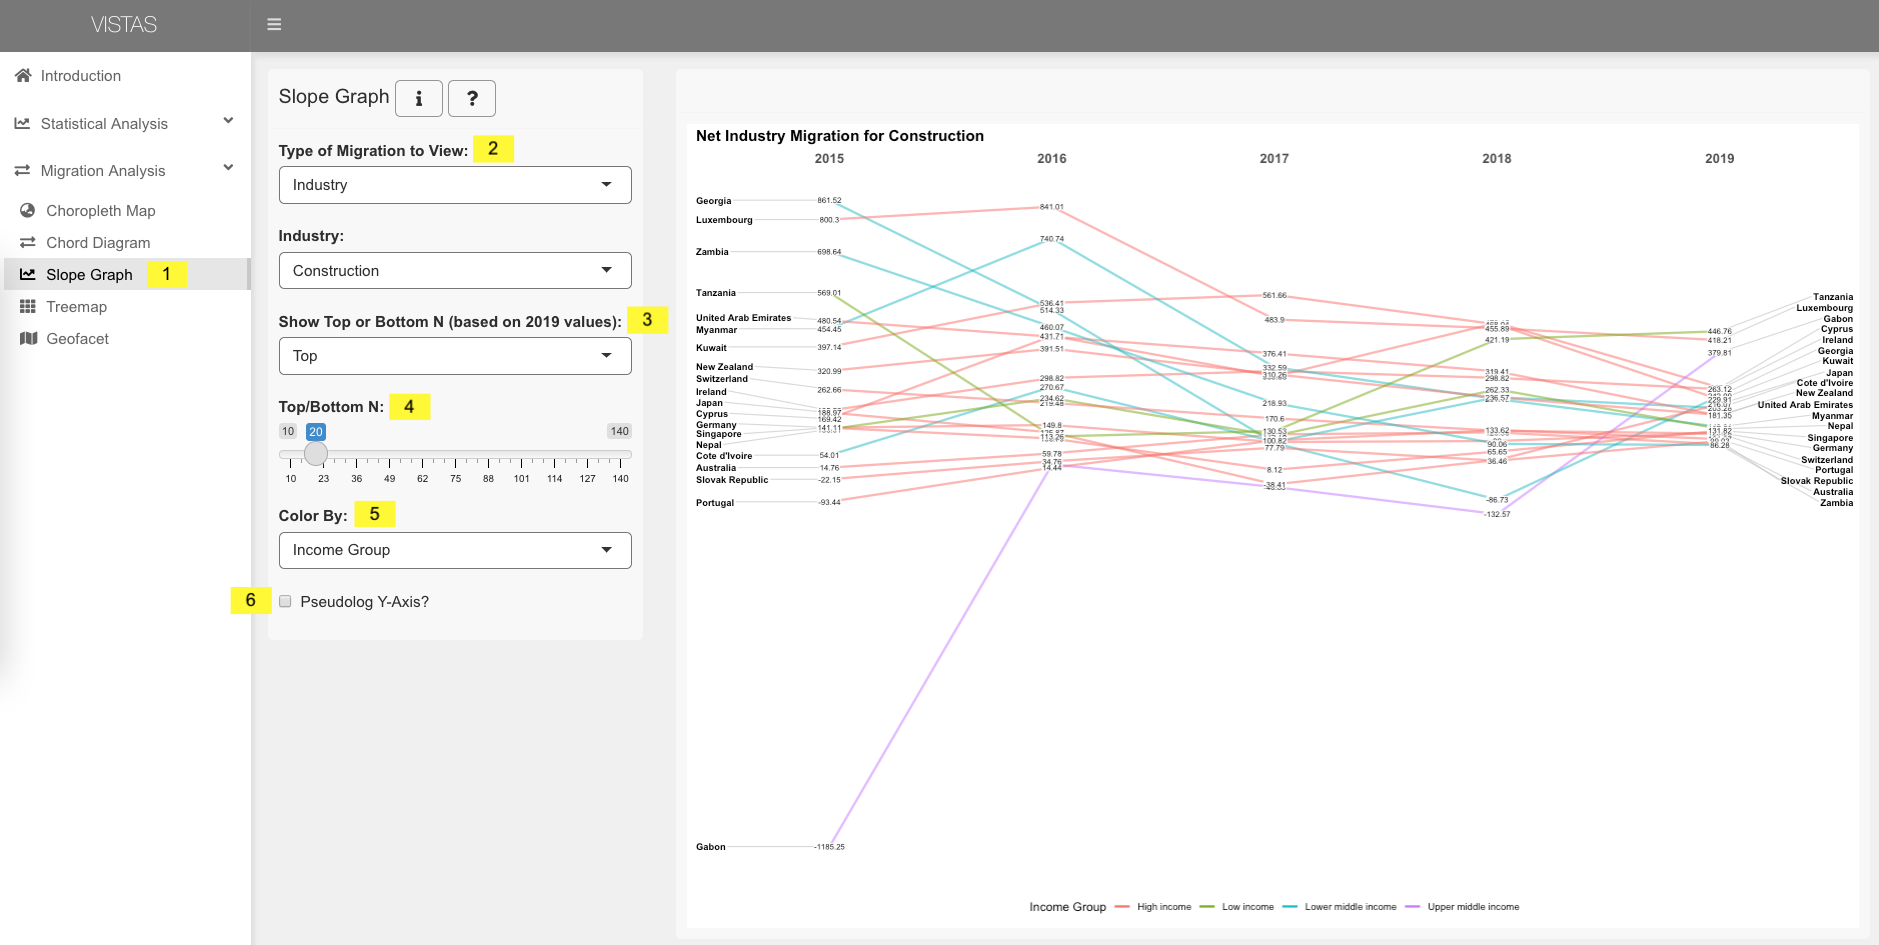
\includegraphics{images/12-slope.png}

\begin{enumerate}
\def\labelenumi{\arabic{enumi}.}
\item
  Click on Slope Graph in the navigation bar.
\item
  Select Type of Migration to View from the dropdown -- Country,
  Industry or Skill.

  \begin{itemize}
  \item
    When Country is selected, you must further select Base Country
    i.e.~the country you want to see the net migration for. The dropdown
    list is sorted by Region then alphabetical order.
  \item
    When Industry is selected, you must further select the Industries
    you want to see the net migration for.
  \item
    When Skills is selected, you must further select the Skills you want
    to see the net migration for.
  \end{itemize}
\item
  Select Top, Bottom or Top and Bottom.

  \begin{itemize}
  \tightlist
  \item
    When ``Top and Bottom'' is selected, both the top and bottom ranked
    countries are shown.
  \end{itemize}
\item
  Indicate the number of countries (N) you want to see on your slope
  graph.
\item
  Select Colour by Region or Income Group. This variable determines the
  colors of the lines on the slope graph.
\item
  Check Pseudolog Y-Axis to transform the y-axis. Pseudolog allows for a
  log-like transformation for both negative and positive values on the
  slope graph; visually, this feature results in lines on the slope
  graph being less cluttered.
\end{enumerate}

\hypertarget{treemap}{%
\paragraph{3.4 Treemap}\label{treemap}}

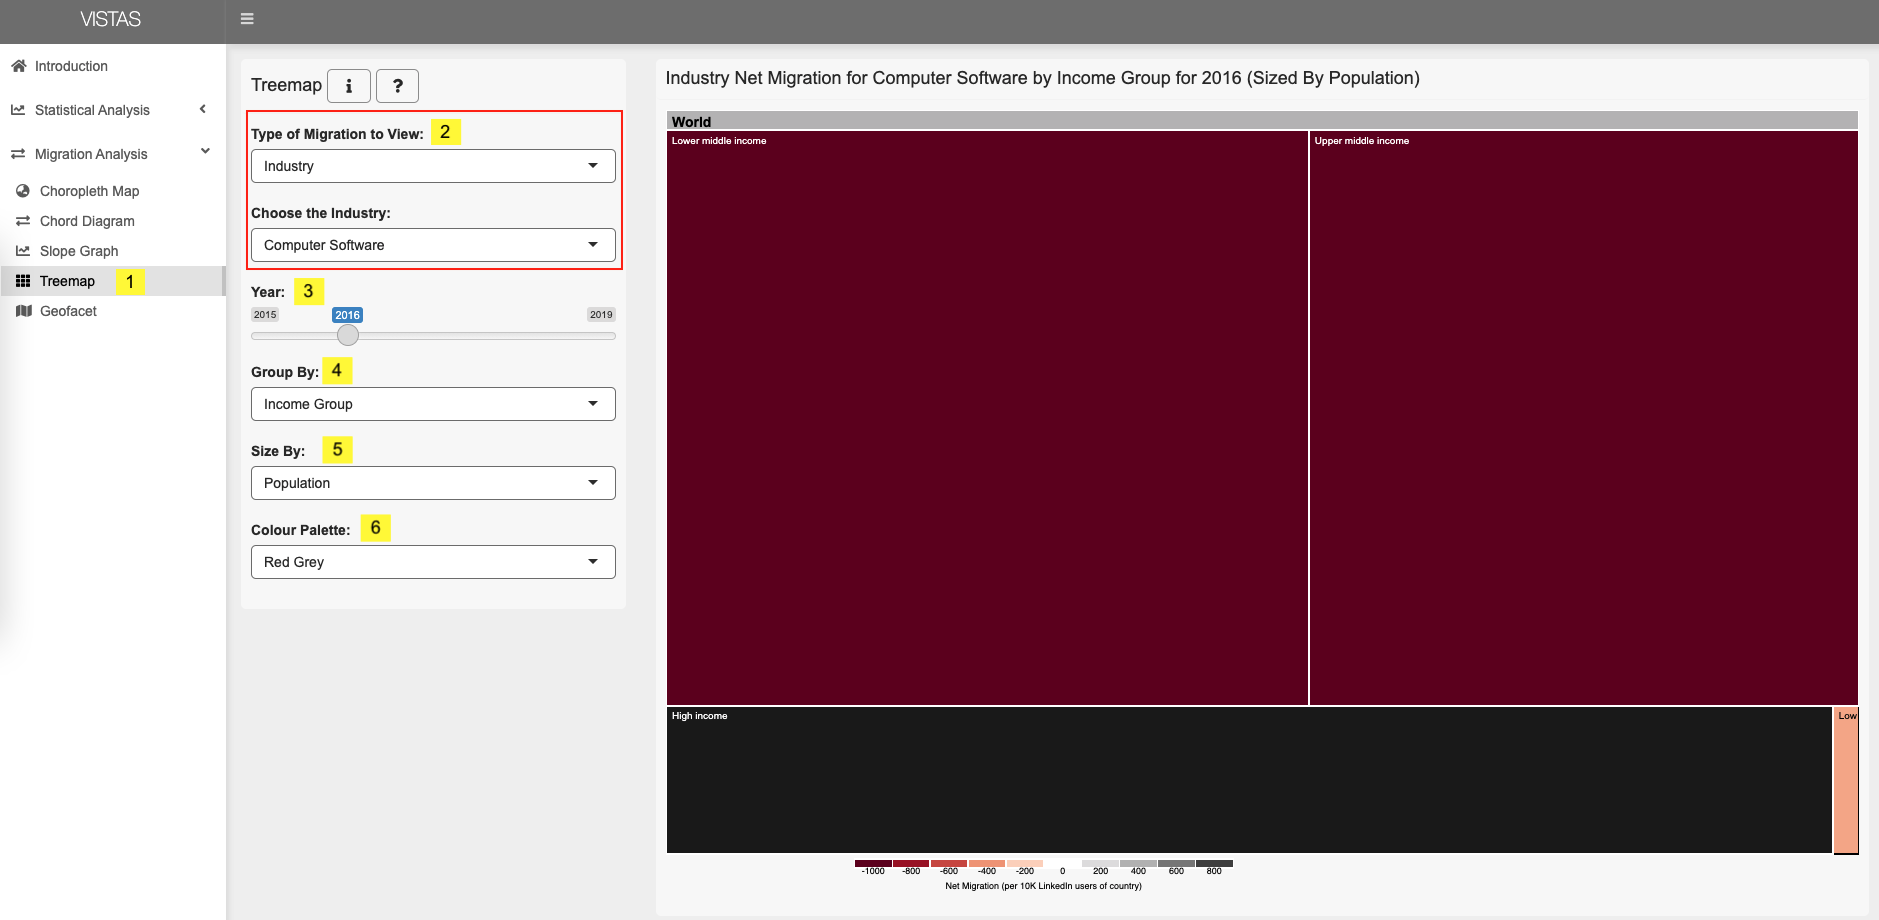
\includegraphics{Images/14-tree.png}

\begin{enumerate}
\def\labelenumi{\arabic{enumi}.}
\item
  Click on Treemap in the navigation bar.
\item
  Select Type of Migration to View from the dropdown -- Country,
  Industry or Skill.

  \begin{itemize}
  \item
    When Country is selected, you must further select Base Country
    i.e.~the country you want to see the net migration for. The dropdown
    list is sorted by Region then alphabetical order.
  \item
    When Industry is selected, you must further select the Industries
    you want to see the net migration for.
  \item
    When Skills is selected, you must further select the Skills you want
    to see the net migration for.
  \end{itemize}
\item
  Select Year on the slider as the data covers years 2015 -- 2019 (both
  years included).
\item
  Select Group by Region or Income Group to see the hierarchy in the
  treemap. Click on the rectangles to go down a level in the hierarchy,
  click on the top header to go up a level in the hierarchy.
\item
  Select Size By Population or GDP Per Capita. This determines the size
  of the rectangles in the treemap.
\item
  Select Colour Palette to watch the colours of the choropleth map
  change.
\end{enumerate}

\hypertarget{geofacet}{%
\paragraph{3.5 Geofacet}\label{geofacet}}

The geofacet has two types of visualisations, line graph and bar graphs.
These graphs are shown based on the user inputs.

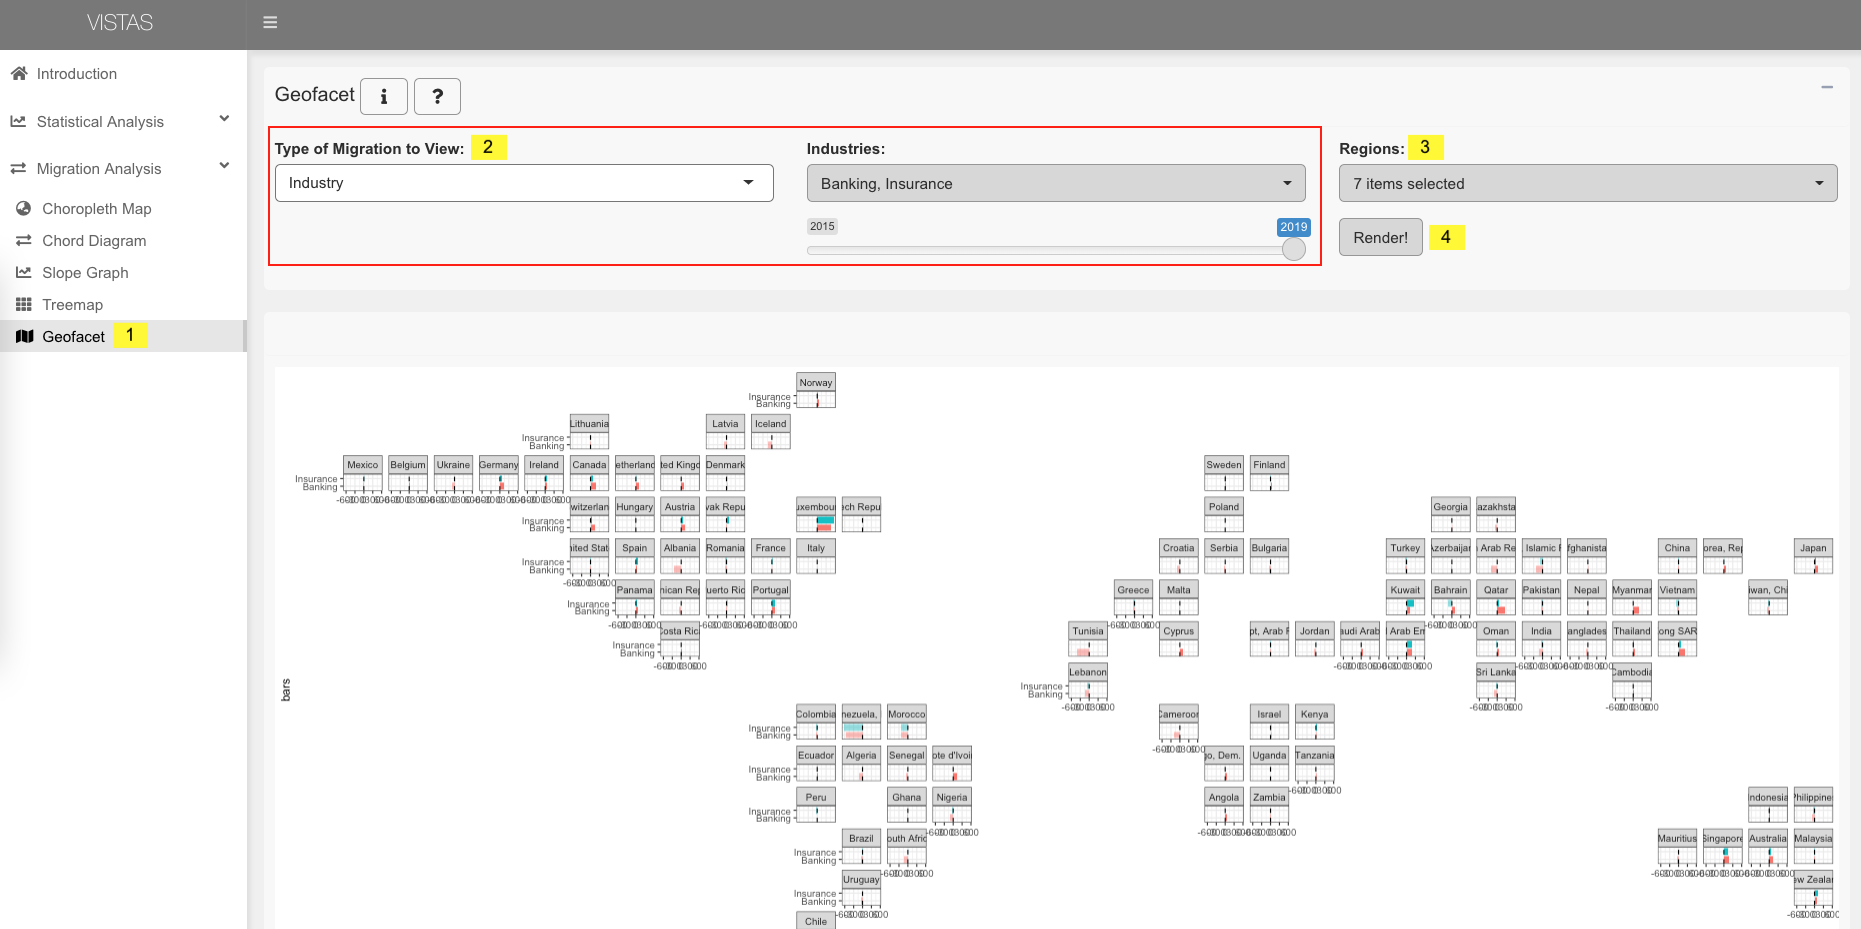
\includegraphics[width=1\textwidth,height=\textheight]{Images/13-facet-bar.png}

\begin{enumerate}
\def\labelenumi{\arabic{enumi}.}
\item
  Click on Geofacet in the navigation bar.
\item
  Select Type of Migration to View from the dropdown -- Country,
  Industry or Skill.

  \begin{itemize}
  \tightlist
  \item
    When Country is selected, you must further select Base Country
    i.e.~the country you want to see the net migration for. The dropdown
    list is sorted by Region then alphabetical order.
  \item
    When Industry is selected, you must further select the Industries
    you want to see the net migration for.
  \item
    When Skills is selected, you must further select the Skills you want
    to see the net migration for.
  \end{itemize}

  If one country, industry or skill is selected, a line chart will show
  the migration trend over the years.

  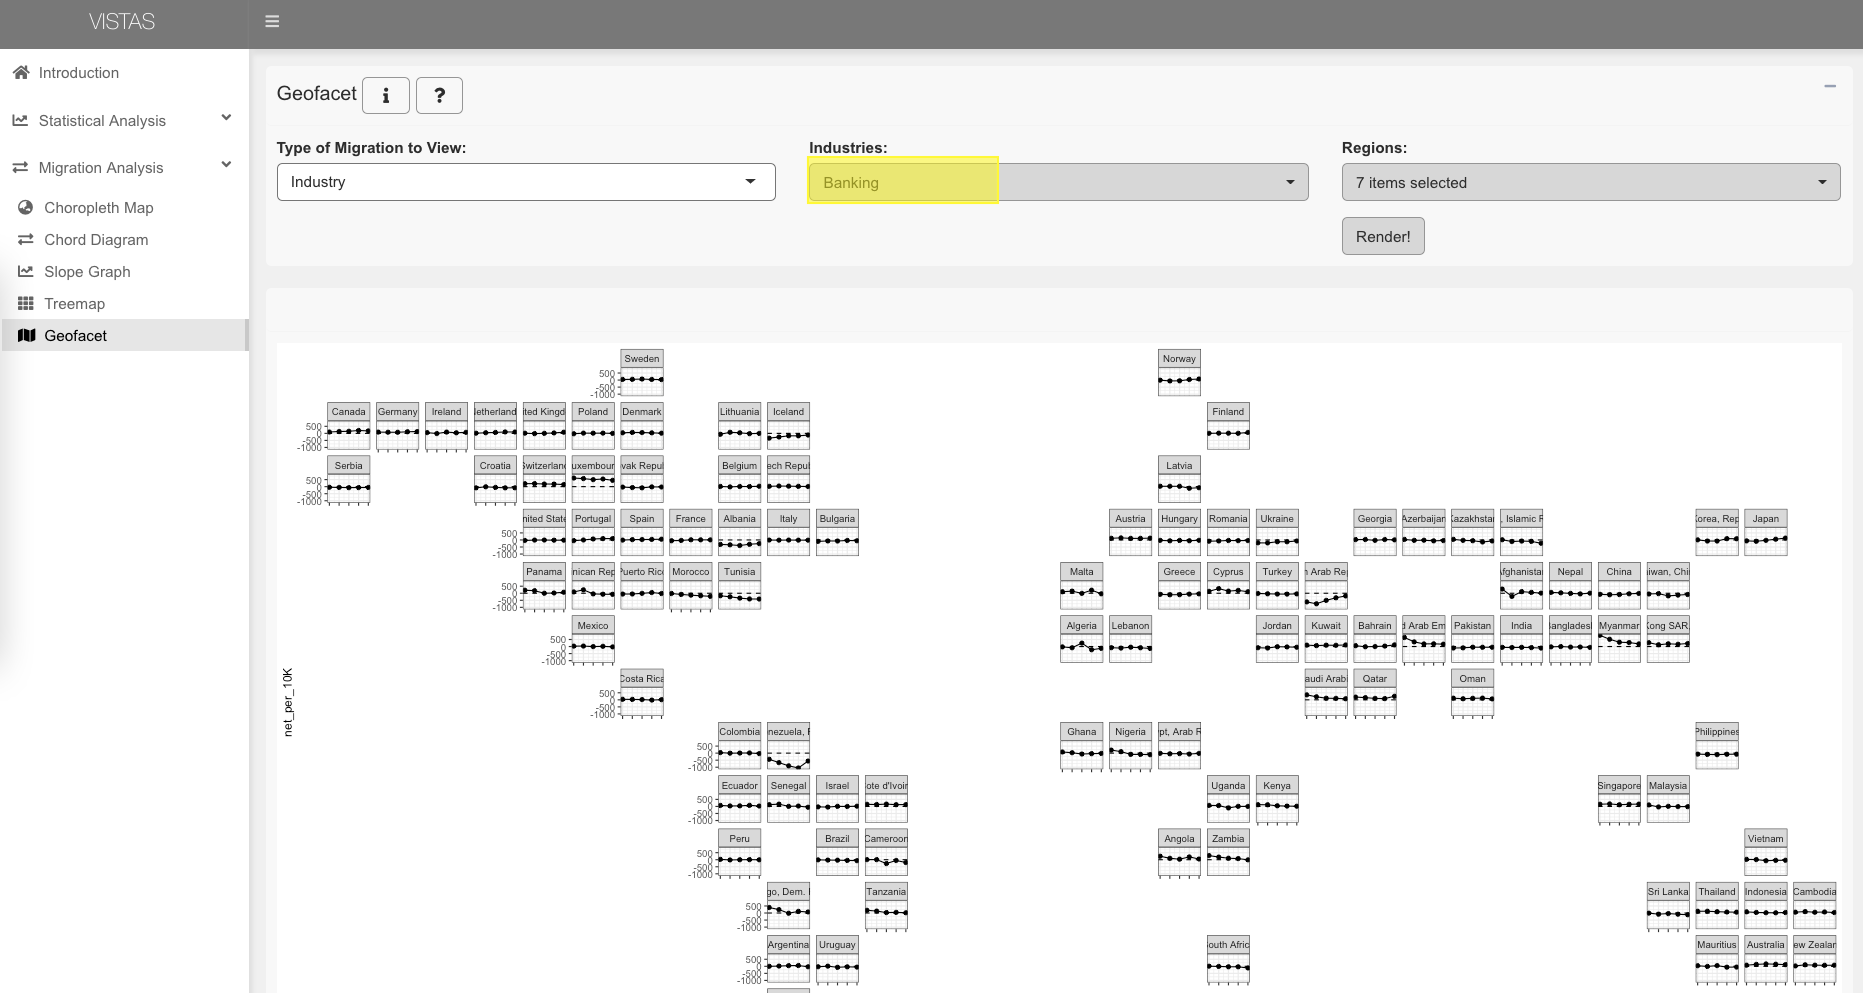
\includegraphics[width=0.8\textwidth,height=\textheight]{Images/13-facet-line.png}

  If more than one country, industry or skills are selected, the bar
  chart will display the migration for them for a selected year.

  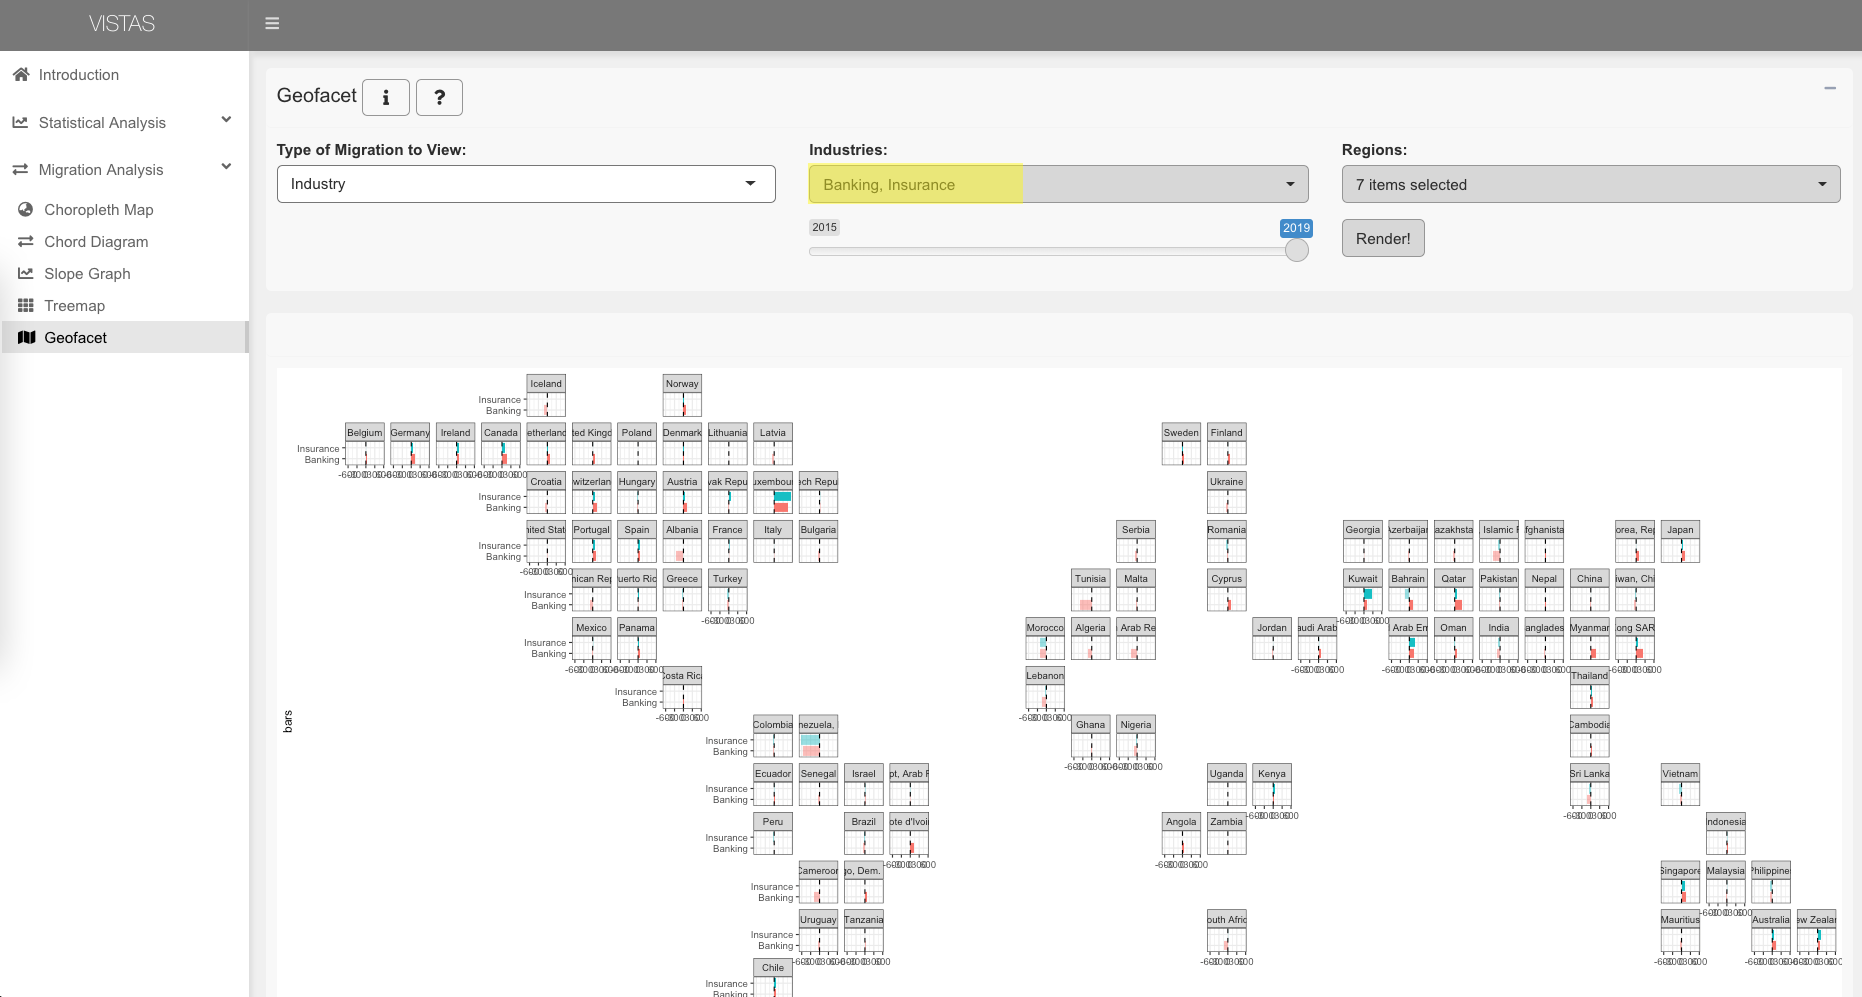
\includegraphics[width=0.8\textwidth,height=\textheight]{Images/13-facet-bar-without-annotations.png}
\item
  Select the Region(s) you would like to see geofacets for. The select
  region(s) will show on the visualization.
\item
  Once you have selected the above, click on ``Render!''. The spinning
  wheel indicates that the geofacets are loading. Once completed, the
  visualization will show.
\item
  To reset your selections for Industry migration and Skills migration,
  go to Type of Migration to View, select country, then the industries
  and skills that you've selected will reset. Then repeat Steps 2-4
  again.
\end{enumerate}

\end{document}
